\chapter{Evaluation} 

% - Weight vs current consumption vs distance
% - Measure start motor overhead and average consumption (show graph?)

\subsection{Energy harvesting from RF}
%TODO explain that the it's more efficient to remove the wisp energy harvester and only use the one on the robot
Small modifications have been made to the WISP to allow the energy harvester on the robot to harvest energy from RF.
The energy harvester, the storage capacitor and the diode to bypass the harvester, were removed from a WISP.
A wire was soldered to the input pin pad of the now removed harvester on the WISP PCB.
This wire was connected directly to the input of the harvester on the robot.

To evaluate the time required for the robot to harvest enough energy a small experiment was done.
Energy was provided to the WISP on the robot trough an Impinj Speedway R1000 RFID reader, which was connected to a Laird antenna.
The robot was placed 20cm away from the antenna, typically the distance where the most energy is harvested.
On average the robot required 48 seconds fully charge and move away from the reader.

\section{Performance in different light conditions}

% Temperature
% Light intensity
% No difference between the heatlamps in power consumed
% Halogen distributes the light more even
% Panel from nuna
% 

To evaluate the charge-time of the robot a comparison was m
Energy is harvested from a light.
However 



\begin{figure}
	\centering
	\begin{subfigure}[b]{0.60\textwidth}
		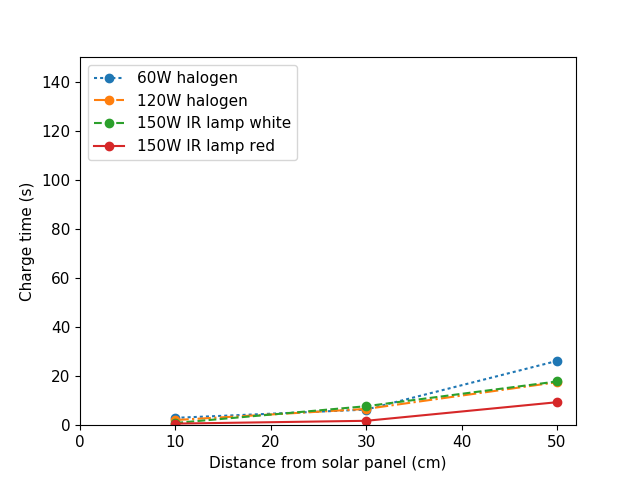
\includegraphics[width=\textwidth]{pics/light_experiment_figure1.png}
		\caption{Ebay 17\% Mono-Si 40x30}
		\label{fig:light_exp1}
	\end{subfigure}

	\begin{subfigure}[b]{0.60\textwidth}
		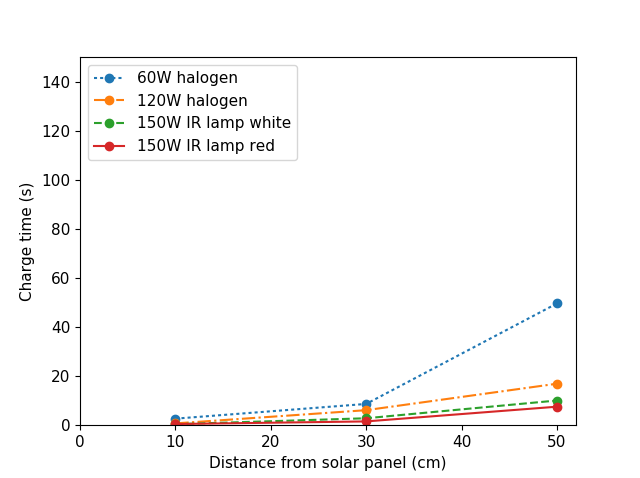
\includegraphics[width=\textwidth]{pics/light_experiment_figure2.png}
		\caption{IXYS SLMD121H04L-ND 20\% Mono-Si 2x 43x14}
		\label{fig:light_exp2}
	\end{subfigure}

	\begin{subfigure}[b]{0.60\textwidth}
		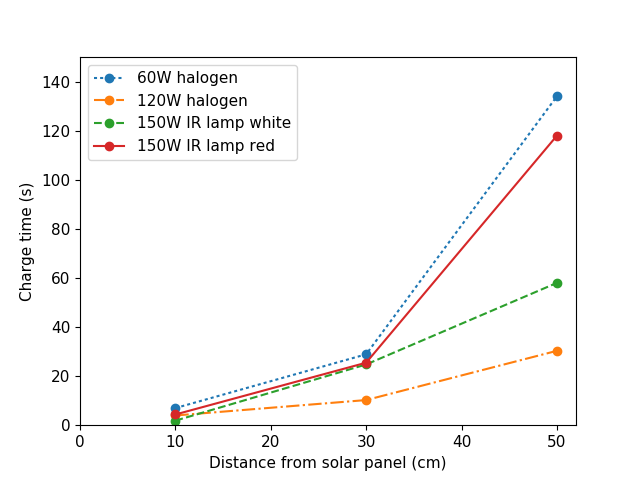
\includegraphics[width=\textwidth]{pics/light_experiment_figure3.png}
		\caption{Azurspace 3G28C 28\% Triple Junction GaAs 80x40}
		\label{fig:light_exp3}
	\end{subfigure}
	\caption{The performance of three different solar panels for different distances from different light sources. The data charge times for the last two are normalized with respect to the surface covered by the first panel.}
\end{figure}

% Casestudy of conditions robot 

% outdoors/indoors/varying light sources/varying solar panels

\section{Controlled movements}

% Comparison deadreckoning accuracy of battery powered robot with solar powered robot

% Try at least one more supercapacitor: 10mF
% Study reducing the frequency of power interrupts ie smaller energy buffer.
% How does this effect the accuracy of locomotion?

% Study the effect of checkpoint frequency on the straight and turn accuracy + combination
% Before and after counting in case of current robot

% Video of robot movement

